\documentclass{article}
\usepackage{polski}
\usepackage[utf8]{inputenc}
\usepackage{graphicx}
\usepackage{tabto}
\usepackage{hyperref}
%s\usepackage[margin=2.5cm]{geomtry}

\usepackage{graphicx}    % Pakiet pozwalający ,,wklejać'' grafikę...
\usepackage{subcaption}
\usepackage{amsmath,amssymb,amsfonts,amsthm,mathtools}
                               % Dołączamy zestaw różnych przydatnych znaczków ...
\DeclareMathOperator{\arccosh}{arccosh}
% dane autora
\author{Wiktor Pilarczyk}
\title{Warsztaty - L6 - SK\\\large{Prowadzący: Tomasz Wierzbicki}}
\date{\today}
% początek dokumentu
\begin{document}
\maketitle
Komputer został skonfigurowany zgodnie z poleceniami zadania.
\section{Część 1.}
\subsection{Co dzieje się, kiedy dodajesz jakiś wpis?}
Zostają wysłane odpowiednie żądania i odpowiedzi.
\subsection{Dlaczego przeglądarka wyświetla w pasku stanu komunikat Waiting for sieci.ii.uni.wroc.pl a odpowiedni wpis nie został dodany?}
Komunikat jest wyświetlany, ponieważ czeka na odpowiedź od serwera, ale my ,,przechwyciliśmy" zapytanie przez co, nie dostaje odpowiedzi, a z tego wynika dlaczego nie zmieniła się zawartość strony.
\subsection{Co zapisał ten program do pliku http request?}
W pliku znajduje się nasze żądanie.
\subsection{Ręczne wysłanie żądania}
Po komendzie "nc -q 3 sieci.ii.uni.wroc.pl 80 < http request" odpowiedni komunikat został dodany, również przy zmianie treści żądania.
\newpage
\section{Część 2.}

Za pomocą komendy - dig A www.debian.org otrzymujemy adres ip przypisany do domeny - 130.89.148.77


Następnie w jednej konsoli wykonujemy - (while true; do netstat -tan | grep 130.89.148.77 ; done) | tee tcp\_log), a w drugiej - wget 130.89.148.77


\begin{figure}[!htb]
\centering
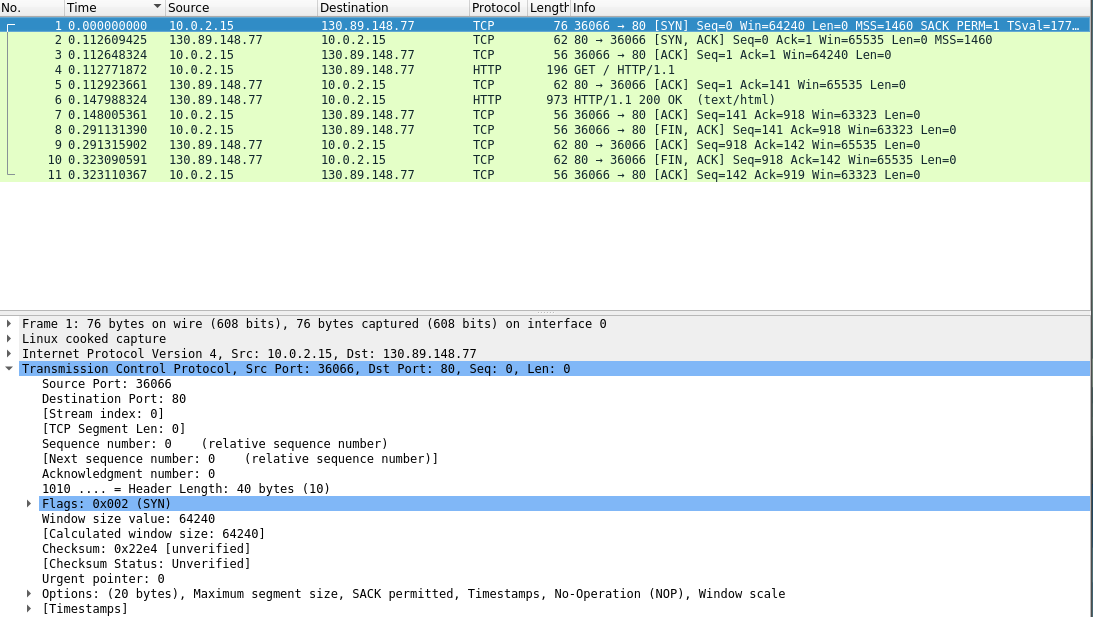
\includegraphics[width=11cm,height=5cm]{info.png}
\caption{Otrzymane pakiety}
\end{figure}

Większość odpowiedzi jest na podstawie powyższego zdjęcia.

\subsection{Jakie gniazda tworzone są do pobierania pliku przez HTTP?}
Gniazda strumieniowe.
\subsection{Jaki jest port źródłowy a jaki docelowy połączenia?}
Z naszego punktu widzenia port źródłowy to 36066, a docelowy 80.
\subsection{Jakie z flag SYN / ACK / FIN są włączone dla danego segmentu?}
Rodzaj flag widzimy w sekcji info każdego segmentu.
\subsection{Które bajty (strumienia danych protokołu HTTP) są przesyłane w segmencie?}
Za pomocą SEQ mówimy, które bajty przesyłamy.
\subsection{Które bajty strumienia danych są potwierdzane danym segmentem?}
Za pomocą ACK potwierdzamy, do którego momentu mamy otrzymane dane.
\subsection{Na podstawie diagramu stanów TCP. Które z tych stanów są widoczne w pliku tcp\_log?}
SYN\_SENT, ESTABLISHED, FIN\_WAIT2, TIME\_WAIT.
\subsection{Która strona wykonuje otwarcie aktywne, a która zamknięcie aktywne?}
Klient - my wykonujemy otwarcie aktywne i zamknięcie aktywne.

\end{document}
